% Standalone manuscript. Compile: pdflatex twice (manual thebibliography).
\documentclass[11pt]{article}
\usepackage[a4paper,margin=2.2cm]{geometry}
\usepackage[utf8]{inputenc}
\usepackage[round,authoryear]{natbib}
\usepackage{booktabs,amsmath,amssymb,mhchem,graphicx,caption,microtype,setspace,array}
\usepackage{tikz}\usetikzlibrary{arrows.meta,positioning,fit,backgrounds}
\setstretch{1.03}
\captionsetup{font=small,labelfont=bf}
\title{\vspace{-1.0cm}\textbf{Early silicification, not oxygenation, governed the preservation of
microfossil morphology across the Great Oxidation Event}}
\author{[Author Name]\\
\small\textit{[Affiliation]}}
\date{}
\begin{document}
\maketitle

\begin{abstract}
\noindent The diversification of morphologically diagnostic microfossils after the Great Oxidation
Event (GOE; $\sim$2.4~Ga) is widely read as a biological signal, yet low atmospheric oxygen before
the GOE should, in principle, have slowed the oxidative degradation of organic matter and favoured
preservation. Compilation of published petrographic, spectroscopic and isotopic data for chert-hosted
biotas on either side of the GOE shows that morphological fidelity tracks the timing and completeness
of early silicification rather than any measure of bottom-water oxygenation. Within the 1.88~Ga
Gunflint biota, morphospecies that preserve internal cellular contents carry $10^{8}$--$10^{9}$
intracellular Fe atoms~$\mu$m$^{-3}$, whereas empty sheaths remain at the matrix background
($\sim$10$^{6}$), documenting a within-assemblage covariation of cellular fidelity with early
mineralization. The silica cycle did not change across the GOE: Precambrian seawater was saturated
with respect to amorphous silica throughout, and silica was not drawn down until the much later
radiation of biosilicifiers. Neither does the sulfur isotope record support a clean redox control on
preservation; the sulfate rise it registers began in the Neoarchean and bears on the decay of organic
matter rather than on the silicification that gates cellular fidelity. The biomarker evidence once
taken to place eukaryotes and cyanobacteria before the GOE is now regarded as contamination.
Morphological richness across the GOE is therefore most parsimoniously interpreted as a facies signal
conditioned by silicification, and the post-GOE ``rise'' of microfossils cannot be read as a
biological radiation without accounting for this preservational structure.
\end{abstract}

\noindent\textbf{Keywords:} Great Oxidation Event; taphonomy; silicification; Archaean--Proterozoic;
microfossils; iron speciation; molecular clocks.

\section{Introduction}

It has long been recognised that anoxia should retard the degradation of sedimentary organic matter,
and that the destruction of cellular morphology during early decay proceeds more slowly where
molecular oxygen is scarce \citep{Canfield1994,Hedges1995}. From this premise one might expect the
Archaean ocean, in which dissolved oxygen was negligible \citep{Pavlov2002} and sulfate scarce
\citep{Habicht2002,Crowe2014}, to have been a favourable setting for the preservation of organic-walled
microfossils. The rock record appears to say the opposite. Morphologically simple, mat-related
carbonaceous remains are present locally in Archaean successions, but assemblages of taxonomically
diagnostic microfossils become abundant and widespread only after the Great Oxidation Event
\citep{Javaux2018,Wacey2014}. The contrast is exemplified by the gunflintiacean biotas of the
$\sim$1.88~Ga Gunflint Iron Formation, which preserve filaments, spheroids and spindle-shaped forms
in cellular detail \citep{Lepot2017}, against the kerogenous globules and rare filaments of the
$\sim$2.72~Ga Tumbiana Formation \citep{Lepot2009}.

Two interpretations of this pattern are routinely advanced. The first is biological: oxygenic
photosynthesis, or the eukaryotic cell, radiated after the GOE, and the record documents that
diversification. The second is preservational: the conditions required to preserve morphology became
more widely available, so that pre-existing diversity simply became visible. The two are not mutually
exclusive, but the distinction matters. If the latter contributes substantially, first-appearance
data cannot be taken at face value as a record of origination.

This paper assembles the relevant published petrographic, spectroscopic and isotopic evidence for
chert-hosted biotas spanning the GOE and asks what governs the preservation of cellular morphology
across that interval. The synthesis points to early silicification, rather than oxygenation, as the
decisive variable, and carries direct consequences for how the early fossil record is read.

\section{Background}

\subsection{Redox across the GOE}

The disappearance of mass-independent sulfur isotope fractionation (S-MIF) between $\sim$2.45 and
2.32~Ga fixes the GOE as the interval in which atmospheric \ce{O2} rose irreversibly above
$\sim$$10^{-5}$ of the present atmospheric level \citep{Holland2006,Bekker2004,Pavlov2002,Farquhar2000}. The
transition was protracted and regionally diachronous \citep{Lyons2014,Philippot2018}. Iron
speciation, the principal local redox proxy, indicates that anoxic ferruginous conditions dominated
deposition throughout the Archaean and much of the Proterozoic
\citep{Canfield1998,Poulton2005,Poulton2011},
euxinia being spatially restricted \citep{Reinhard2009}. Seawater sulfate rose across the GOE from
micromolar to millimolar levels \citep{Habicht2002,Kah2004,Crowe2014}, but the sulfur isotope
evidence for this rise extends into the Neoarchean \citep{Reinhard2009}, and trace-metal and sulfur
isotopic signals of oxidative weathering are now known to predate the GOE in several basins
\citep{Anbar2007}.

\subsection{The microfossil record}

The Archaean record of cellular morphology is sparse and contested. The filamentous structures
described from the $\sim$3.46~Ga Apex chert \citep{Schopf1993} were reinterpreted as abiogenic
\citep{Brasier2002}, and although better-preserved Archaean microbiotas are known from the
$\sim$3.4~Ga Strelley Pool Formation \citep{Sugitani2010,Delarue2020}, they remain modest in
comparison with the post-GOE assemblages. Gunflint-type biotas, with their distinctive filaments and
spheroids, are widespread in shallow-marine cherts of $\sim$1.9~Ga age and permit taxonomic
discrimination \citep{Javaux2018}. The post-GOE increase in the diversity and abundance of
morphologically recognisable microfossils is the pattern that invites explanation.

\subsection{The silica cycle}

Before the evolution of silica-biomineralising organisms, the ocean was saturated or
supersaturated with respect to amorphous silica. Silica concentrations of order $\sim$2~mM, two to
three orders of magnitude above the modern value, are inferred for Archaean and Proterozoic seawater,
with abiological precipitation the dominant sink \citep{Siever1992,Perry2003}; the role of early
silicification in exceptional preservation extends into the Neoproterozoic \citep{Tarhan2016}. The drawdown of
seawater silica was driven by the much later radiation of sponges, radiolaria and ultimately
diatoms, and is essentially a Neoproterozoic to Phanerozoic phenomenon. The capacity for early
silica precipitation was therefore available on both sides of the GOE.

\section{Material and approach}

Six chert-hosted biotas were compared (Table~\ref{tab:panel}): the Strelley Pool Formation, the
Moodies Group and the Tumbiana Formation (pre-GOE), and the Belcher Group, the Gunflint Iron
Formation and the Sokoman Iron Formation (post-GOE). These units span shallow-marine to
peri-tidal silicified facies of comparable, low metamorphic grade, allowing the influence of
thermal maturity to be held approximately constant. For each, published descriptions of petrography,
Raman spectroscopy of carbonaceous material, iron mineralogy and sulfur geochemistry were compiled;
no new measurements are reported. Where published constraints are absent, that is stated rather than
inferred.

The strongest single line of evidence is drawn from nanoscale petrography of the Gunflint biota
\citep{Lepot2017}, in which the relationship between cellular preservation and early mineralization
can be assessed quantitatively and within a single assemblage, avoiding the facies-averaging that
limits between-formation comparison.

\begin{table}[t]
\centering\small
\caption{Preservation of cellular morphology in six chert-hosted biotas across the GOE. Grades are
qualitative summaries of the cited literature.}
\label{tab:panel}
\begin{tabular}{p{0.18\linewidth}p{0.10\linewidth}p{0.16\linewidth}p{0.30\linewidth}p{0.14\linewidth}}
\toprule
Unit (age) & GOE & Facies / maturity & Preservation of morphology & Silicification \\
\midrule
Strelley Pool ($\sim$3.4~Ga) & pre & chert; Raman $\sim$300$^\circ$C & diverse (lenticular, spinose, ``tail-like'') but of lower cellular fidelity than Gunflint; walls partly silica-replaced & early \\
Moodies Gp ($\sim$3.22~Ga) & pre & siliciclastic tidal; low grade & tufted and cavity-dwelling mats; cellular detail poorly resolved & weak \\
Tumbiana Fm ($\sim$2.72~Ga) & pre & stromatolitic carbonate/chert; $<$300$^\circ$C & abundant kerogenous globules; rare filaments; no cellular assemblage & weak \\
\midrule
Belcher Gp ($\sim$2.0~Ga) & post & chert-replaced stromatolites; low grade & diverse microbiota, chert-permineralised & early \\
Gunflint Fm ($\sim$1.88~Ga) & post & chert; prehnite--pumpellyite & diverse, high cellular fidelity; intracellular Fe-silicate/carbonate & early \\
Sokoman IF ($\sim$1.88~Ga) & post & chert; low grade & Gunflint-type assemblage & early \\
\bottomrule
\end{tabular}
\\[2pt]
\raggedright\footnotesize Sources: \citep{Sugitani2010,Delarue2020,Wacey2012,Homann2015,Lepot2009,%
Decreane2021,Lepot2017,Wacey2013,Alleon2016,Javaux2018}.
\end{table}

\section{The control on morphological fidelity}

\subsection{Within-assemblage evidence from Gunflint}

At the scale of individual microfossil populations, the Gunflint biota shows that the preservation of
internal cellular structure is coupled to early mineralization. Morphospecies retaining cellular
contents, including thick-walled \emph{Huroniospora} and Type-2 \emph{Gunflintia}, carry between
$3\times10^{8}$ and $10^{9}$ intracellular Fe atoms~$\mu$m$^{-3}$, together with finer
intra-microfossil quartz than the surrounding matrix \citep{Lepot2017}. Empty sheaths, in contrast,
including Type-1 \emph{Gunflintia minuta}, \emph{Animikiea} and thin-walled \emph{Huroniospora}, are
depleted in iron to the level of the chert matrix background ($\sim$$1.5\times10^{6}$~atoms~$\mu$m$^{-3}$;
Fig.~\ref{fig:gunflint}). Whether the intracellular iron reflects in vivo biomineralization or very
early diagenetic precipitation, its restriction to morphospecies with preserved contents indicates
that cellular fidelity required mineral entombment before decay had destroyed internal structure.

\begin{figure}[t]
\centering
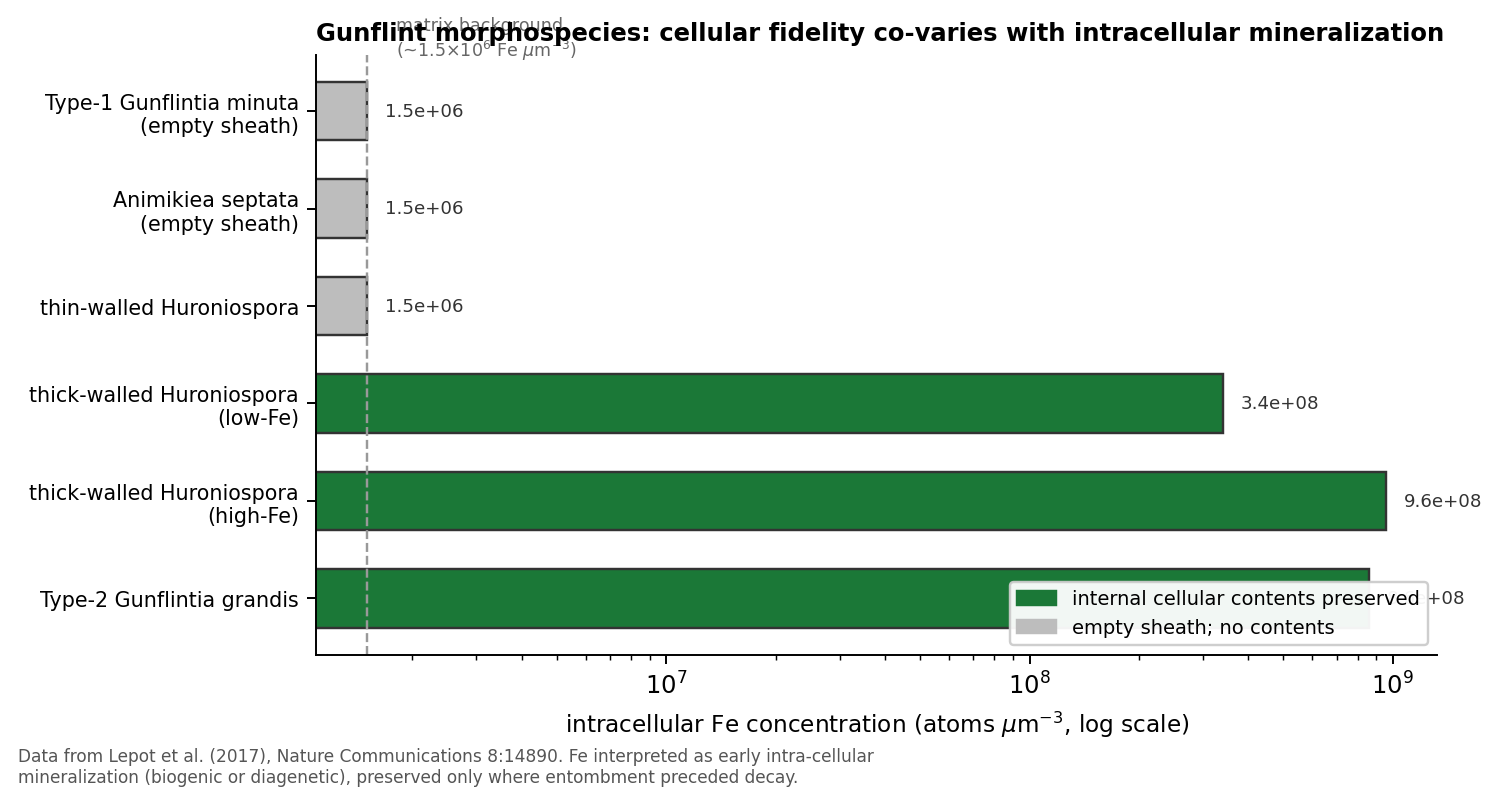
\includegraphics[width=0.92\linewidth]{fig_gunflint.png}
\caption{Intracellular Fe concentration in Gunflint morphospecies, against the preservation of
cellular contents. Morphospecies with preserved internal structure carry $10^{8}$--$10^{9}$~Fe
atoms~$\mu$m$^{-3}$; empty sheaths remain at the matrix background. Data from \citet{Lepot2017}.}
\label{fig:gunflint}
\end{figure}

A focused-ion-beam comparison of the Strelley Pool and Gunflint biotas reached a compatible
conclusion at the between-assemblage scale \citep{Wacey2012}: although the Strelley Pool
microfossils are morphologically diverse, their cellular fidelity is lower than that of Gunflint,
with wall organic matter partly replaced by silica. Morphological diversity and cellular fidelity are
therefore not the same quantity, and both are graded with the timing and completeness of
silicification.

\subsection{Between-assemblage pattern}

Across the six units, the preservation of cellular morphology tracks the quality of early
silicification, independently of position relative to the GOE (Table~\ref{tab:panel}). The
pre-GOE Strelley Pool biota, where silicification was early and complete, preserves a diverse
morphological assemblage, whereas the pre-GOE Tumbiana and Moodies biotas, in which silicification
was weak or confined to mat textures, preserve kerogen and mats rather than cells. The post-GOE
Gunflint, Sokoman and Belcher biotas are all early-silicified and morphologically rich. Pyrite, where
present, is a poor indicator of fidelity: in Gunflint, pyritisation is confined to patches, develops
under locally sulfate-limited conditions, and destroys rather than preserves organic structure
\citep{Wacey2013,Lepot2017}. Pyritisation is also documented in pre-GOE Tumbiana stromatolites
\citep{Decreane2021}, so it cannot mark a post-GOE preservational threshold.

\subsection{Why redox and the silica cycle cannot supply a GOE control}

If a change in redox across the GOE had governed morphological preservation, the proxy record of that
change should align with the palaeontological pattern. It does not. Iron speciation indicates
pervasive ferruginous deposition on both sides of the GOE \citep{Poulton2011}, and the sulfur
isotope signal of rising sulfate extends back into the Neoarchean \citep{Reinhard2009,Philippot2018}.
The sulfate rise registered by $\delta^{34}$S bears on microbial sulfate reduction and the
sulfurisation of organic matter, a pathway that affects the survival of bulk kerogen rather than the
templating of cellular morphology. The relevant control on morphology, the availability of early
silica, was unchanging across the GOE: Precambrian seawater remained silica-saturated throughout, and
the silica cycle was not reorganised until the much later appearance of biosilicifiers
\citep{Siever1992,Perry2003}.

\section{Origins, first appearances, and the limits of inference}

If the post-GOE increase in morphological diversity reflects, even in part, the unmasking of lineages
that existed but were not previously preserved, then independent temporal evidence should place
those lineages before the GOE. Molecular clock analyses now place the stem origin of cyanobacteria,
and with it oxygenic photosynthesis, in the Archaean, at $\sim$3.3--3.6~Ga \citep{Sanchez2021},
whereas the crown-group diversification of extant Oxyphotobacteria is estimated to postdate the rise
of oxygen \citep{Shih2017}. Molecular clock estimates for the last eukaryotic common ancestor remain
model-dependent and scattered, but several precede the first widely accepted eukaryotic
microfossils, leaving a protracted gap between molecular and palaeontological estimates of
divergence \citep{Betts2018,Eme2014} (Fig.~\ref{fig:clocks}).

\begin{figure}[t]
\centering
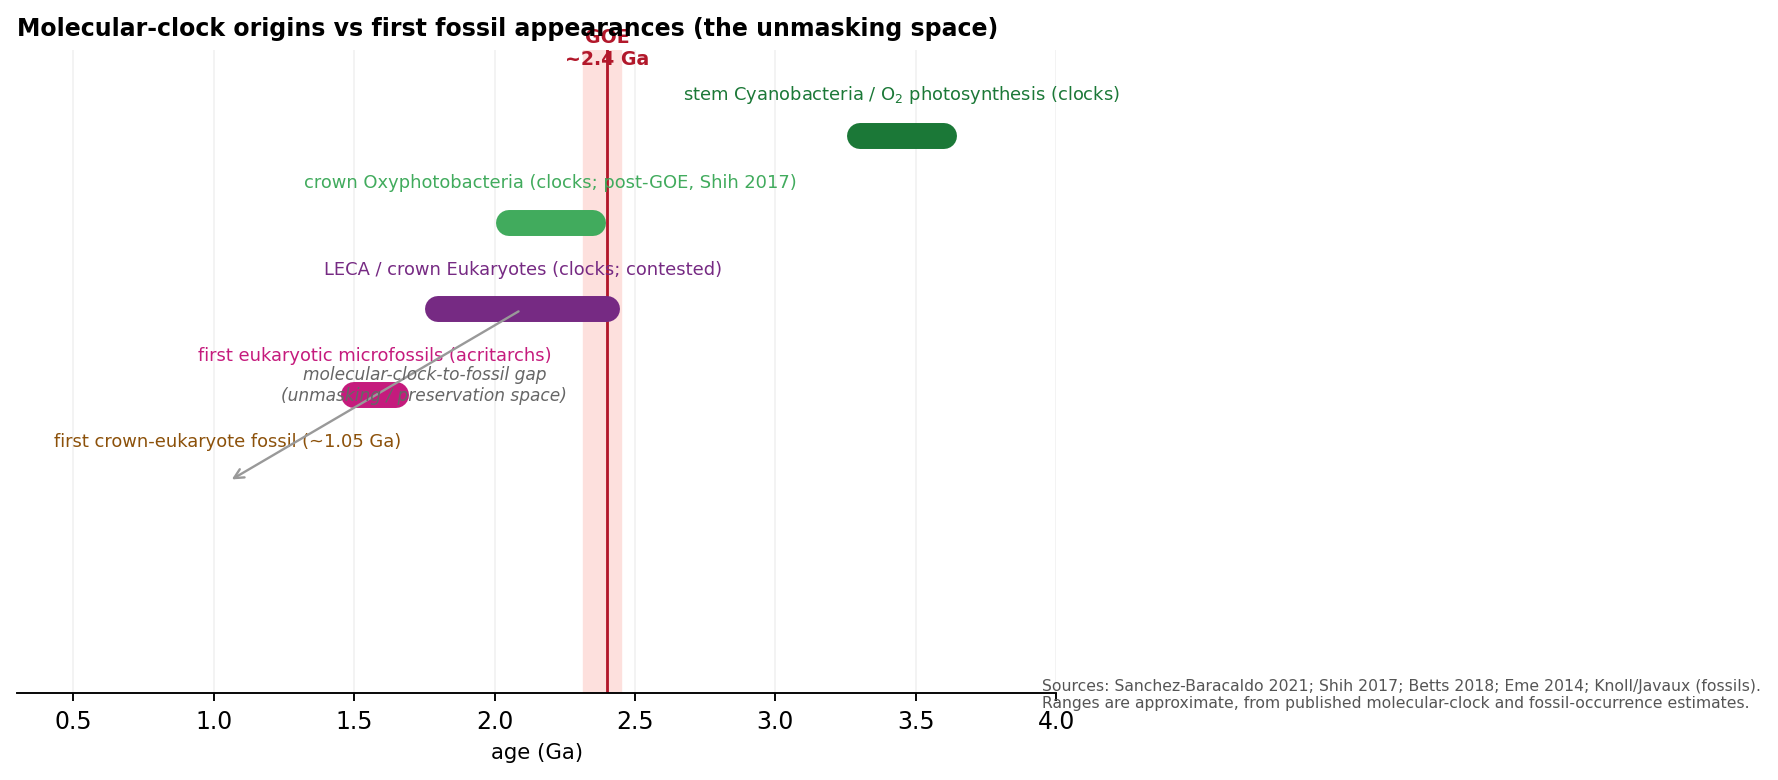
\includegraphics[width=\linewidth]{fig_v3_timeline.png}
\caption{Molecular clock estimates of lineage origin against first fossil appearances. The stem
origin of cyanobacteria lies in the Archaean \citep{Sanchez2021}; crown Oxyphotobacteria diversify
around or after the GOE \citep{Shih2017}; eukaryote molecular-clock estimates precede the first
widely accepted eukaryotic fossils \citep{Betts2018,Eme2014}. Ranges are approximate.}
\label{fig:clocks}
\end{figure}

The biomarker record cannot at present resolve this gap. The steranes and 2-methylhopanes reported
from $\sim$2.7~Ga shales, once taken as evidence for Archaean eukaryotes and cyanobacteria
\citep{Brocks1999}, were shown to reside in younger carbonate veins \citep{Rasmussen2008}, and
analysis of ultraclean drill cores has demonstrated that hopane and sterane concentrations in
Archaean rocks are indistinguishable from procedural blanks \citep{French2015}. The molecular fossil
evidence for pre-GOE eukaryotes and oxygenic photosynthesis must therefore be regarded as
contaminant.

The consequence is a logical bind. First-appearance data are themselves the preservational signal
under examination, and the biomarker evidence that might have provided an independent check is
contaminated. The question of whether the post-GOE pattern reflects evolution or unmasking cannot be
settled from the rock record alone, but the uncertainty runs in one direction: molecular clocks are
consistent with lineages that predate the GOE, and a facies control on preservation is sufficient to
account for their late appearance. Reading the post-GOE diversification as a biological radiation, in
the absence of correction for preservation, is not warranted.

\section{Discussion}

The compiled evidence supports a single, consistent reading. The preservation of cellular morphology
in Precambrian cherts is conditioned by early silicification, a facies and early-diagenetic variable
that operated throughout the Archaean and Proterozoic but was expressed unevenly, depending on the
silica budget of the depositional environment and the timing of cementation relative to decay. Where
silica entombment was early and complete, as at Gunflint and, to a lesser degree, Strelley Pool,
morphology survives in cellular detail; where it was weak or absent, as at Tumbiana and Moodies, only
kerogen and mat textures remain (Fig.~\ref{fig:model}). Oxygenation, and the sulfate rise that
accompanied it, modified the decay of organic matter and the sulfurisation of kerogen
\citep{Lepot2009,Decreane2021} but did not gate the silicification on which cellular fidelity
depends.

\begin{figure}[t]
\centering
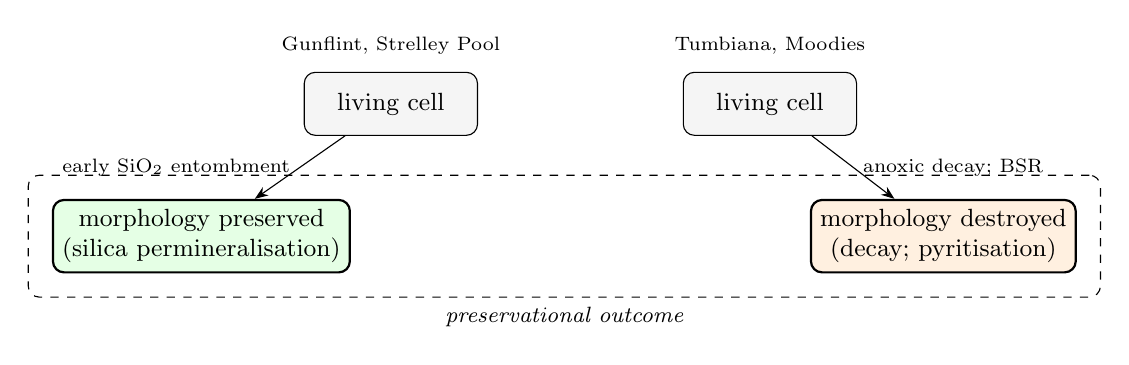
\begin{tikzpicture}[>=Stealth, node distance=6mm and 10mm,
  cell/.style={draw,rounded corners,align=center,fill=gray!8,minimum width=22mm,minimum height=8mm,font=\small},
  outc/.style={draw,thick,rounded corners,align=center,minimum width=30mm,minimum height=9mm,font=\small},
  every node/.style={font=\small}]
\node[cell] (c1) {living cell};
\node[cell,right=26mm of c1] (c2) {living cell};
\node[outc,below left=8mm and -6mm of c1, fill=green!10] (m1) {morphology preserved\\(silica permineralisation)};
\node[outc,below right=8mm and -6mm of c2, fill=orange!12] (m2) {morphology destroyed\\(decay; pyritisation)};
\node[draw,dashed,rounded corners,fit=(m1)(m2),inner sep=3mm,label={[font=\footnotesize\itshape]below:preservational outcome}] {};
\draw[->] (c1) -- node[left,font=\scriptsize]{early \ce{SiO2} entombment} (m1);
\draw[->] (c2) -- node[right,font=\scriptsize]{anoxic decay; BSR} (m2);
\node[above=1mm of c1,font=\scriptsize,align=center]{Gunflint, Strelley Pool};
\node[above=1mm of c2,font=\scriptsize,align=center]{Tumbiana, Moodies};
\end{tikzpicture}
\caption{Preservational pathways. Where early silica permineralisation outpaces decay, cellular
morphology is retained; where decay (and pyritisation) precedes or accompanies mineralization,
morphology is lost and only kerogen survives. The balance is set by depositional facies and the
timing of cementation, not by the oxygenation state of ambient water.}
\label{fig:model}
\end{figure}

This reading carries several implications. First, abundance and diversity counts compiled across the
GOE cannot be interpreted as proxies for biomass or evolutionary innovation without correction for
the silicification available in the sampled facies; the well-exposed and intensively sampled
gunflint-type cherts of the Palaeoproterozoic are liable to over-represent the biology of their time
relative to less completely silicified Archaean successions. Second, the gap between molecular clock
estimates of origination and the first appearance of fossils, most conspicuously for eukaryotes
\citep{Betts2018}, is consistent with a preservational lag and need not denote a late evolutionary
origin. Third, for the search for biosignatures on Mars and in other ancient successions, the
relevant variable for the preservation of morphology is a silica-precipitating facies, not the
presence of oxygen.

The principal limitation is that the comparison rests on a synthesis of published petrographic
descriptions rather than a uniform new dataset. The within-Gunflint relationship between intracellular
iron and cellular fidelity \citep{Lepot2017} is quantitative, but the between-formation pattern is
semi-quantitative and would be strengthened by a standardised, per-population scoring of
silicification and fidelity measured under identical conditions on matched samples. A regression of
morphological fidelity on a quantitative silicification index, within single formations of comparable
thermal maturity, would convert the inference advanced here into a direct test, and would do so with
greater power than any comparison couched as a two-group contrast across the GOE.

\section{Conclusions}

Across the GOE, the preservation of microfossil morphology in Precambrian cherts is governed by
early silicification. Within the Gunflint biota, cellular fidelity co-varies quantitatively with
intracellular mineralization; between biotas, fidelity tracks the quality of silicification and is
independent of position relative to the GOE. The silica cycle did not change across the GOE, the
sulfur isotope evidence for the sulfate rise extends into the Neoarchean and bears on organic-matter
decay rather than on morphological templating, and the biomarker evidence for pre-GOE eukaryotes and
cyanobacteria is best regarded as contaminant. The post-GOE diversification of morphologically
diagnostic microfossils is therefore most parsimoniously read as a facies signal, conditioned by
silicification, and should not be interpreted as a biological radiation without preservational
correction. A within-formation, quantitative test of fidelity against silicification is the
appropriate next step.

%==================================================================
\bibliographystyle{plainnat}
\begin{thebibliography}{99}\footnotesize\linespread{0.95}\selectfont\setlength{\itemsep}{0pt}\setlength{\parskip}{0pt}
\bibitem[Alleon et al.(2016)]{Alleon2016} Alleon, J., Bernard, S., Le Guerr\'{o}u\'{e}, N., et al.\
(2016). Molecular preservation of 1.88~Ga Gunflint organic microfossils as a function of temperature
and mineralogy. \textit{Nature Communications} 7, 11977.
\bibitem[Anbar et al.(2007)]{Anbar2007} Anbar, A.~D., Duan, Y., Lyons, T.~W., et al.\ (2007). A whiff
of oxygen before the Great Oxidation Event? \textit{Science} 317, 1903--1906.
\bibitem[Bekker et al.(2004)]{Bekker2004} Bekker, A., Holland, H.~D., Wang, P.-L., et al.\ (2004).
Dating the rise of atmospheric oxygen. \textit{Nature} 427, 117--120.
\bibitem[Betts et al.(2018)]{Betts2018} Betts, H.~C., Puttick, M.~N., Clark, J.~W., et al.\ (2018).
Integrated genomic and fossil evidence illuminates life's early evolution and eukaryote origin.
\textit{Nature Ecology \& Evolution} 2, 1556--1562.
\bibitem[Brasier et al.(2002)]{Brasier2002} Brasier, M.~D., Green, O.~R., Jephcoat, A.~P., et al.\
(2002). Questioning the evidence for Earth's oldest fossils. \textit{Nature} 416, 76--81.
\bibitem[Brocks et al.(1999)]{Brocks1999} Brocks, J.~J., Logan, G.~A., Buick, R., \& Summons, R.~E.\
(1999). Archean molecular fossils and the early rise of eukaryotes. \textit{Science} 285, 1033--1036.
\bibitem[Canfield(1994)]{Canfield1994} Canfield, D.~E. (1994). Factors influencing organic carbon
preservation in marine sediments. \textit{Chemical Geology} 114, 315--329.
\bibitem[Canfield(1998)]{Canfield1998} Canfield, D.~E. (1998). A new model for Proterozoic ocean
chemistry. \textit{Nature} 396, 450--453.
\bibitem[Crowe et al.(2014)]{Crowe2014} Crowe, S.~A., D{\o}ssing, L.~N., Beukes, N.~J., et al.\
(2014). Sulfate was a trace constituent of the Archean ocean. \textit{Science} 346, 735--739.
\bibitem[Decreane et al.(2021)]{Decreane2021} Decreane, S., Philippot, P., Ader, M., et al.\ (2021).
Intense biogeochemical iron cycling revealed in Neoarchean Tumbiana Formation stromatolites.
\textit{Geochimica et Cosmochimica Acta}.
\bibitem[Delarue et al.(2020)]{Delarue2020} Delarue, F., Robert, F., Derenne, S., et al.\ (2020). Out
of rock: a new look at the morphological and geochemical preservation of microfossils from the
3.46~Gyr-old Strelley Pool Formation. \textit{Precambrian Research} 336, 105472.
\bibitem[Eme et al.(2014)]{Eme2014} Eme, L., Sharpe, S.~C., Brown, M.~W., \& Roger, A.~J.\ (2014). On
the age of eukaryotes: evaluating evidence from fossils and molecular clocks. \textit{Cold Spring
Harbor Perspectives in Biology} 6, a016139.
\bibitem[Farquhar et al.(2000)]{Farquhar2000} Farquhar, J., Bao, H., \& Thiemens, M.\ (2000).
Atmospheric influence of Earth's earliest sulfur cycle. \textit{Science} 289, 756--758.
\bibitem[French et al.(2015)]{French2015} French, K.~L., Hallmann, C., Hope, J.~M., et al.\ (2015).
Reappraisal of hydrocarbon biomarkers in Archean rocks. \textit{Proceedings of the National Academy
of Sciences} 112, 5915--5920.
\bibitem[Habicht et al.(2002)]{Habicht2002} Habicht, K.~S., Gade, M., Thamdrup, B., Berg, P., \&
Canfield, D.~E.\ (2002). Calibration of sulfate levels in the Archean ocean. \textit{Science} 298,
2372--2374.
\bibitem[Hedges \& Keil(1995)]{Hedges1995} Hedges, J.~I., \& Keil, R.~G.\ (1995). Sedimentary organic
matter preservation: an assessment and speculative synthesis. \textit{Marine Chemistry} 49, 81--115.
\bibitem[Holland(2006)]{Holland2006} Holland, H.~D.\ (2006). The oxygenation of the atmosphere and
oceans. \textit{Philosophical Transactions of the Royal Society B} 361, 903--915.
\bibitem[Homann et al.(2015)]{Homann2015} Homann, M., Heubeck, C., Airo, A., \& Tice, M.~M.\ (2015).
Morphological adaptations of 3.22~Ga-old tufted microbial mats to Archean coastal--habitat
(Moodies Group, Barberton Greenstone Belt). \textit{Precambrian Research} 266, 47--64.
\bibitem[Javaux \& Lepot(2018)]{Javaux2018} Javaux, E.~J., \& Lepot, K.\ (2018). The Paleoproterozoic
fossil record: implications for the evolution of the biosphere during Earth's middle-age.
\textit{Earth-Science Reviews} 176, 68--94.
\bibitem[Kah et al.(2004)]{Kah2004} Kah, L.~C., Lyons, T.~W., \& Frank, T.~D.\ (2004). Low marine
sulfate and protracted oxygenation of the Proterozoic biosphere. \textit{Nature} 431, 834--838.
\bibitem[Lepot et al.(2009)]{Lepot2009} Lepot, K., Benzerara, K., Rividi, N., et al.\ (2009). Organic
matter heterogeneities in 2.72~Ga stromatolites: alteration versus preservation by sulfur
incorporation. \textit{Geochimica et Cosmochimica Acta} 73, 6579--6599.
\bibitem[Lepot et al.(2017)]{Lepot2017} Lepot, K., Addad, A., Knoll, A.~H., et al.\ (2017). Iron
minerals within specific microfossil morphospecies of the 1.88~Ga Gunflint Formation. \textit{Nature
Communications} 8, 14890.
\bibitem[Lyons et al.(2014)]{Lyons2014} Lyons, T.~W., Reinhard, C.~T., \& Planavsky, N.~J.\ (2014).
The rise of oxygen in Earth's early ocean and atmosphere. \textit{Nature} 506, 307--315.
\bibitem[Pavlov \& Kasting(2002)]{Pavlov2002} Pavlov, A.~A., \& Kasting, J.~F.\ (2002).
Mass-independent fractionation of sulfur isotopes in Archean sediments: strong evidence for an anoxic
Archean atmosphere. \textit{Astrobiology} 2, 27--41.
\bibitem[Perry \& Lefticariu(2007)]{Perry2003} Perry, E.~C., \& Lefticariu, P.\ (2007). Formation and
geochemistry of Precambrian cherts. In \textit{Treatise on Geochemistry} (2nd ed.), vol.~7, 99--113.
\bibitem[Philippot et al.(2018)]{Philippot2018} Philippot, P., \'{A}vila, J.~N., Killingsworth, B.~A.,
et al.\ (2018). Globally asynchronous sulphur isotope signals require re-definition of the Great
Oxidation Event. \textit{Nature Communications} 9, 2245.
\bibitem[Poulton \& Canfield(2005)]{Poulton2005} Poulton, S.~W., \& Canfield, D.~E.\ (2005).
Development of a sequential extraction procedure for iron: implications for iron partitioning in
continentally derived particulates. \textit{Chemical Geology} 214, 209--221.
\bibitem[Poulton \& Canfield(2011)]{Poulton2011} Poulton, S.~W., \& Canfield, D.~E.\ (2011).
Ferruginous conditions: a dominant feature of the ocean through Earth's history. \textit{Elements} 7,
107--112.
\bibitem[Rasmussen et al.(2008)]{Rasmussen2008} Rasmussen, B., Fletcher, I.~R., Brocks, J.~J., \&
Kilburn, M.~R.\ (2008). Reassessing the first appearance of eukaryotes and cyanobacteria by
2-Ga-old hydrocarbon biomarkers. \textit{Nature} 455, 1101--1104.
\bibitem[Reinhard et al.(2009)]{Reinhard2009} Reinhard, C.~T., Raiswell, R., Scott, C., Anbar, A.~D.,
\& Lyons, T.~W.\ (2009). A late Archean sulfidic sea stimulated by early oxidative weathering of the
continents. \textit{Science} 326, 713--716.
\bibitem[S\'{a}nchez-Baracaldo(2021)]{Sanchez2021} S\'{a}nchez-Baracaldo, P.\ (2021). The Archean
origin of oxygenic photosynthesis and extant cyanobacterial lineages. \textit{Proceedings of the
Royal Society B} 288, 20210675.
\bibitem[Schopf(1993)]{Schopf1993} Schopf, J.~W.\ (1993). Microfossils of the early Archean Apex
chert: new evidence of the antiquity of life. \textit{Science} 260, 640--646.
\bibitem[Shih et al.(2017)]{Shih2017} Shih, P.~M., Hemp, J., Ward, L.~M., Matzke, N.~J., \& Fischer,
W.~W.\ (2017). Crown group Oxyphotobacteria postdate the rise of oxygen. \textit{Geobiology} 15,
19--29.
\bibitem[Siever(1992)]{Siever1992} Siever, R.\ (1992). The silica cycle in the Precambrian.
\textit{Geochimica et Cosmochimica Acta} 56, 3265--3272.
\bibitem[Sugitani et al.(2010)]{Sugitani2010} Sugitani, K., Lepot, K., Nagaoka, T., et al.\ (2010).
Biogenicity of morphologically diverse carbonaceous microstructures from the ca. 3400~Ma Strelley
Pool Formation, in the Pilbara Craton, Western Australia. \textit{Astrobiology} 10, 899--920.
\bibitem[Tarhan et al.(2016)]{Tarhan2016} Tarhan, L.~G., Hood, A.~v.~S., Droser, M.~L., Gehling, J.~G.,
\& Briggs, D.~E.~G.\ (2016). Exceptional preservation of soft-bodied Ediacara Biota promoted by
silica-rich oceans. \textit{Geology} 44, 951--954.
\bibitem[Wacey et al.(2012)]{Wacey2012} Wacey, D., Menon, S., Green, L., et al.\ (2012). Taphonomy of
very ancient microfossils from the $\sim$3400~Ma Strelley Pool Formation and $\sim$1900~Ma Gunflint
Formation: new insights using a focused ion beam. \textit{Precambrian Research} 220--221, 234--250.
\bibitem[Wacey et al.(2013)]{Wacey2013} Wacey, D., McLoughlin, N., Kilburn, M.~R., et al.\ (2013).
Nanoscale analysis of pyritized microfossils reveals differential heterotrophic consumption in the
$\sim$1.9~Ga Gunflint chert. \textit{Proceedings of the National Academy of Sciences} 110,
8020--8024.
\bibitem[Wacey et al.(2014)]{Wacey2014} Wacey, D., Saunders, M., \& Brasier, M.~D.\ (2014).
Changing the picture of Earth's earliest fossils (3.5--1.9~Ga) with new approaches and discoveries.
\textit{Proceedings of the National Academy of Sciences} 111, 8778.
\end{thebibliography}

\end{document}
